\chapter{Results \& Analysis}

\section{Measurement Results}
In order to obtain variation of channel conditions, measurement of DVB-T signal was taken in two different places, namely TU Delft Library and Poptahof Noord. Some parameters like power level, spectrum, and decision were taken during the measurement. For a starting point, we let the detector automatically choose appropriate threshold value above the average noise level, which is be done by quick scanning a given range of frequencies. Then, the signal scanning process begins from the minimum frequency until the maximum frequency with step value 1 MHz. As the number of measurements is large enough, only several results are shown in Table~\ref{tab:result-table}.

\begin{table}[H]
    \caption{Signal measurement results}
    \label{tab:result-table}
    \resizebox{\textwidth}{!}{%
    \begin{tabular}{|l|p{0.1\textwidth}|p{0.1\textwidth}|p{0.1\textwidth}|p{0.1\textwidth}|p{0.1\textwidth}|p{0.1\textwidth}|p{0.1\textwidth}|p{0.1\textwidth}|p{0.1\textwidth}|}
    \hline
	\multirow{2}{*}{\textbf{User}}		& \textbf{Center}									& \multicolumn{4}{|c|}{\textbf{TU Delft Library (6th floor) (52.002947, 4.375374)}}										& \multicolumn{4}{|c|}{\textbf{Poptahof Noord (4th floor) (51.999881, 4.351265)}}									\\ \cline{3-10} 
										& \textbf{Frequency (MHz)}	             			& \textbf{Level (dB)}   & \textbf{Detected (Th = -72.071 dB)}	& \textbf{Average (dB)}     & \textbf{Std. Deviation} 	& \textbf{Level (dB)}	& \textbf{Detected (Th = -73.5985)} & \textbf{Average (dB)}     & \textbf{Std. Deviation} 	\\ \hline \hline
    NTS3 Bouquet 4 						& 498                    							& -52.220				& Yes									& \multirow{5}{*}{-52.700}  & \multirow{5}{*}{4.038}	& -48.940				& Yes                             	& \multirow{5}{*}{-51.733}	& \multirow{5}{*}{4.789}  	\\ \cline{1-4}\cline{7-8}
    NTS4 Bouquet 5 						& 522                    							& -50.124				& Yes									&               			&							& -43.887				& Yes                             	&               			&               			\\ \cline{1-4}\cline{7-8}
    NTS1 Bouquet 2 						& 698                    							& -55.013				& Yes									&               			&							& -54.064				& Yes                             	&               			&               			\\ \cline{1-4}\cline{7-8}
    RTS Bouquet 1  						& 722                    							& -52.007				& Yes									&               			&							& -54.250				& Yes                             	&               			&               			\\ \cline{1-4}\cline{7-8}
    NTS2 Bouquet 3 						& 762                    							& -61.558				& Yes									&               			&							& -57.526				& Yes                             	&               			&               			\\ \hline
    Empty          						& 586                    							& -77.237				& No 									& \multirow{12}{*}{-75.109} & \multirow{12}{*}{6.671}	& -78.107				& No                              	& \multirow{12}{*}{-76.218}	& \multirow{12}{*}{6.679} 	\\ \cline{1-4}\cline{7-8}
    Empty          						& 607                    							& -77.594				& No 									&							&							& -78.204				& No                              	&              				&               			\\ \cline{1-4}\cline{7-8}
    Empty          						& 621                    							& -76.593				& No 									&							&							& -78.247				& No                              	&              				&               			\\ \cline{1-4}\cline{7-8}
    Empty          						& 633                    							& -78.085				& No 									&							&							& -78.529				& No                              	&              				&               			\\ \cline{1-4}\cline{7-8}
    Empty          						& 642                    							& -77.497				& No 									&							&							& -78.427				& No                              	&              				&               			\\ \cline{1-4}\cline{7-8}
    Empty          						& 673                    							& -77.820				& No 									&							&							& -77.587				& No                              	&              				&               			\\ \cline{1-4}\cline{7-8}
    Empty          						& 730                    							& -77.924				& No 									&							&							& -78.401				& No                              	&              				&               			\\ \cline{1-4}\cline{7-8}
    Empty          						& 782                    							& -77.372				& No 									&							&							& -78.470				& No                              	&              				&               			\\ \cline{1-4}\cline{7-8}
    Empty          						& 792                    							& -47.862				& No 									&							&							& -55.602				& No                              	&              				&               			\\ \cline{1-4}\cline{7-8}
    Empty          						& 813                    							& -56.287				& No 									&							&							& -57.373				& No                              	&              				&               			\\ \cline{1-4}\cline{7-8}
    Empty          						& 841                    							& -77.951				& No 									&							&							& -78.536				& No                              	&              				&               			\\ \cline{1-4}\cline{7-8}
    …              						& …                      							& …        				& …										&							&							& …      				& …                               	&              				&               			\\ \hline
    \end{tabular}}%
\end{table}

From Table~\ref{tab:result-table}, there are 5 registered DVB-T frequencies captured by the detector~\cite{radiotvnederland}. The rest are categorized as empty channels though they could be occupied by other radio systems. We obtain the mean and standard deviation of the level from both detected signals and empty channels to analyze receiver performance (ROC). Note that we set 5 seconds as the duration of measurement per frequency to ensure the stability of the detector, reducing error of measurement.

\section{Signal Detection}

A signal can be detected when its power level is above a threshold value as seen in Figure~\ref{fig:gnu-signal-detect}. In this project, we expand the mechanism of the signal detection by comparing the number of detection in a certain range of frequency with DVB-T bandwidth. In this case, the bandwidth is 8 MHz. Figure~\ref{fig:edge-signal-detect} depicts the edge detection of a DVB-T spectrum that has center frequency of 498 MHz (NTS3 Bouquet 4). One of the edges lies on 494 MHz and another one on 502 MHz, which means that the bandwidth of the detected signal is about 8 MHz and thus can be categorized as DVB-T signal.

% GNU radio signal detection
\begin{figure}[H]
    \centering
    \begin{subfigure}[b]{0.4\textwidth}
        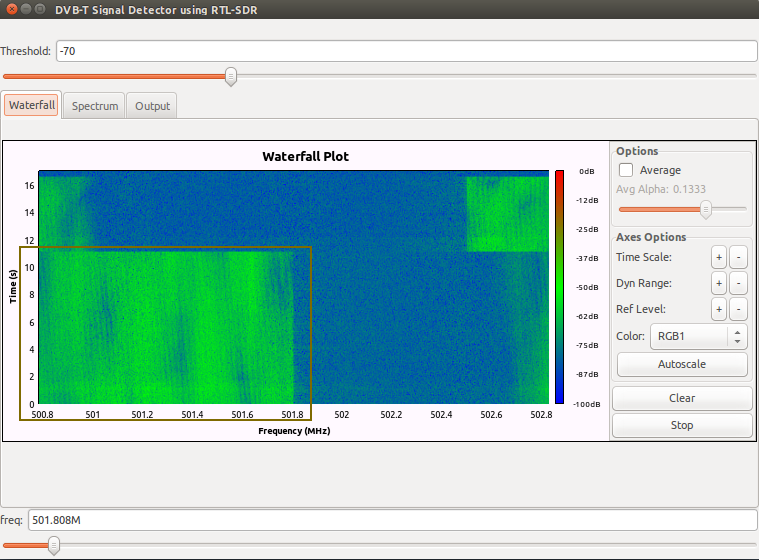
\includegraphics[width=\textwidth]{figures/waterfall-1}
    \end{subfigure}
    ~ %add desired spacing between images, e. g. ~, \quad, \qquad, \hfill etc. 
    %(or a blank line to force the subfigure onto a new line)
    \begin{subfigure}[b]{0.4\textwidth}
        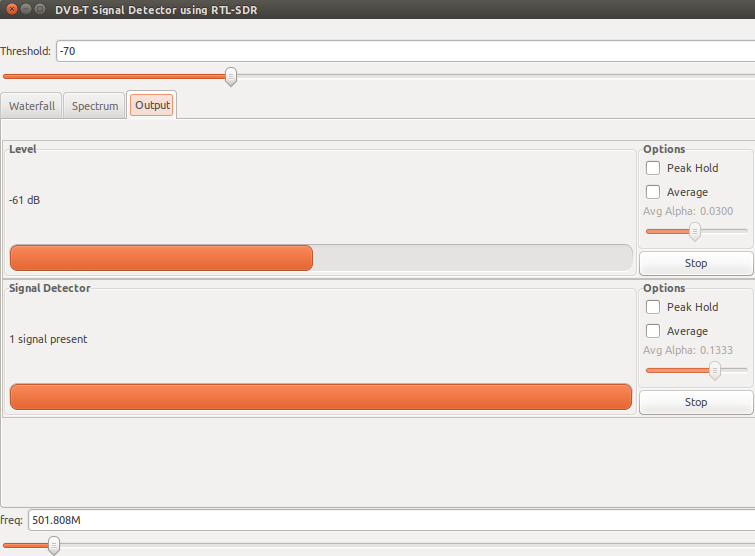
\includegraphics[width=\textwidth]{figures/detection-1}
    \end{subfigure}
    \caption{Waterfall plot and signal detection status}\label{fig:gnu-signal-detect}
\end{figure}

% Signal Detection at 498 MHz
\begin{figure}[H]
    \centering
    \begin{subfigure}[b]{0.4\textwidth}
        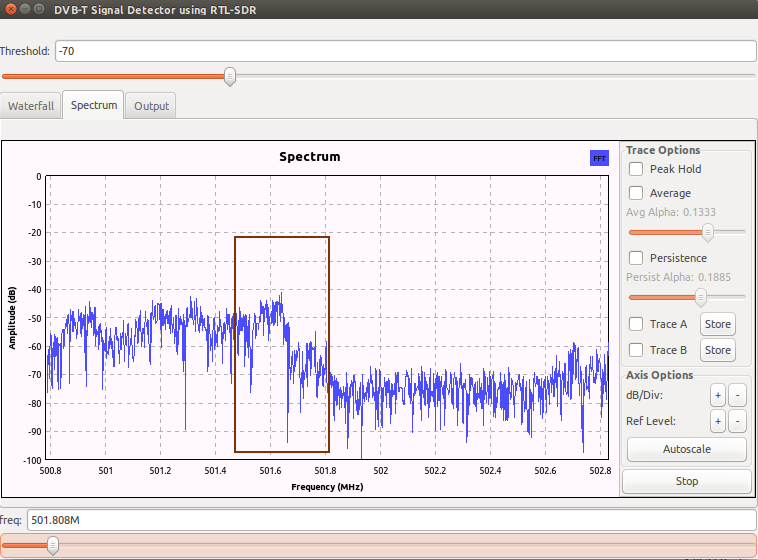
\includegraphics[width=\textwidth]{figures/signal-detect-1}
    \end{subfigure}
    ~ %add desired spacing between images, e. g. ~, \quad, \qquad, \hfill etc. 
    %(or a blank line to force the subfigure onto a new line)
    \begin{subfigure}[b]{0.4\textwidth}
        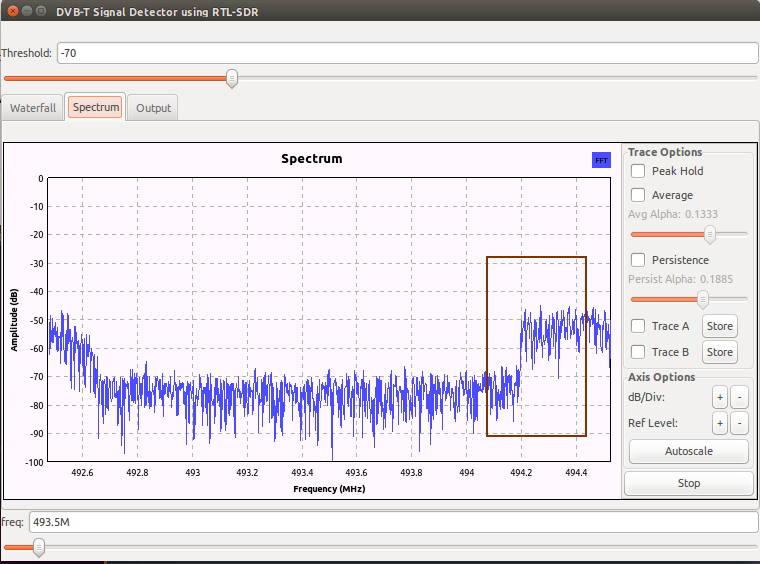
\includegraphics[width=\textwidth]{figures/signal-detect-2}
    \end{subfigure}
    \caption{Edge detection of detected DVB-T signal which has center frequency of 498 MHz}\label{fig:edge-signal-detect}
\end{figure}

By using automated measurement tool that is built with Python script, we are able to plot the measurement of signal level over the whole range of DVB-T frequency spectrum. It can also identify and recognize DVB-T signal based on bandwidth. Figure~\ref{fig:freq-lib-60} shows the spectrum of the signals measured on the given range of frequency, and the recognized DVB-T center frequency with threshold -60 dB captured at TU Delft Library. There are some of signals that could not be detected as they below the threshold value, e.g. the signal at frequency 480 MHz, 550 MHz, and 760 MHz. Therefore, it may lead to the increased probability of misdetection of a signal.

% TU Delft Lib results
\begin{figure}[H]
    \centering
    \begin{subfigure}[b]{0.45\textwidth}
        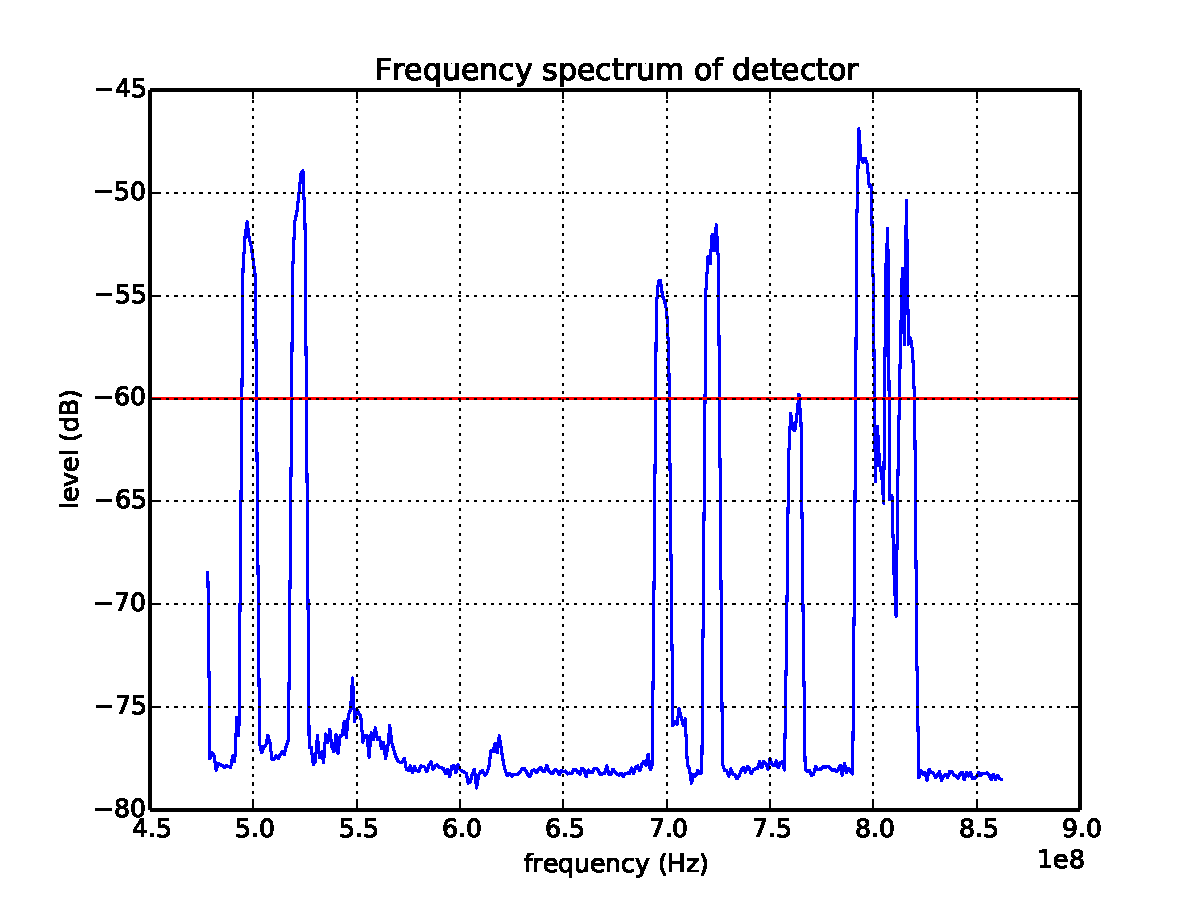
\includegraphics[width=\textwidth]{figures/lib-60-freq}
    \end{subfigure}
    ~ %add desired spacing between images, e. g. ~, \quad, \qquad, \hfill etc. 
    %(or a blank line to force the subfigure onto a new line)
    \begin{subfigure}[b]{0.45\textwidth}
        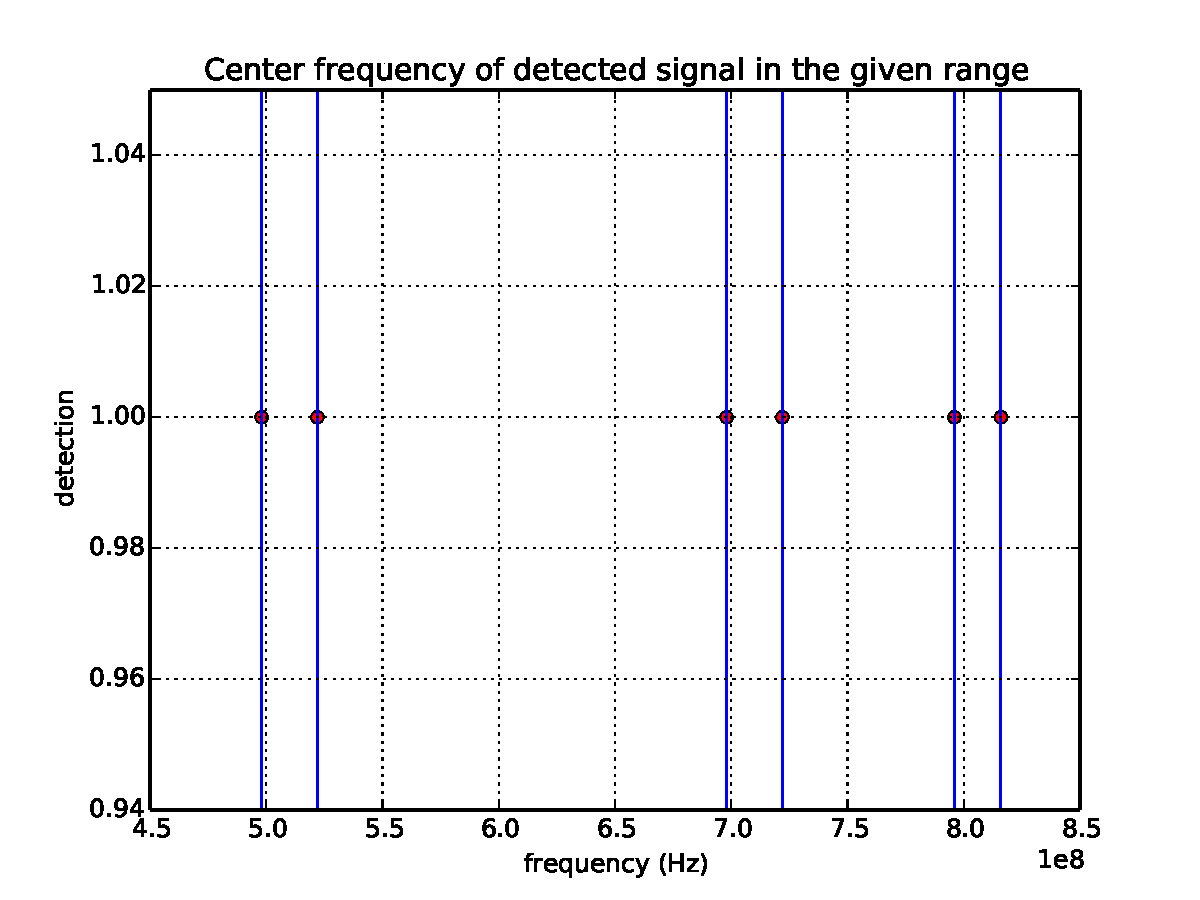
\includegraphics[width=\textwidth]{figures/lib-60-center}
    \end{subfigure}
    \caption{Frequency spectrum of signal with threshold -60 dB captured at TU Delft Library}\label{fig:freq-lib-60}
\end{figure}

One way to reduce the probability of misdetection is by lowering the threshold value. Figure~\ref{fig:freq-lib-auto} shows the frequency spectrum and the detected center frequency of DVB-T signal when the threshold value is lowered to -72.0716 dB by using automatic threshold finder. The signal at 480 MHz is still not detected as DVB-T signal as the bandwidth is not around 8 MHz. This also happens to the signal captured at the range of 790 - 820 MHz in which the detected bandwidth is larger than 8 MHz. Therefore, the detector decides not to include such kind of signals in its detection list.

\begin{figure}[H]
    \centering
    \begin{subfigure}[b]{0.45\textwidth}
        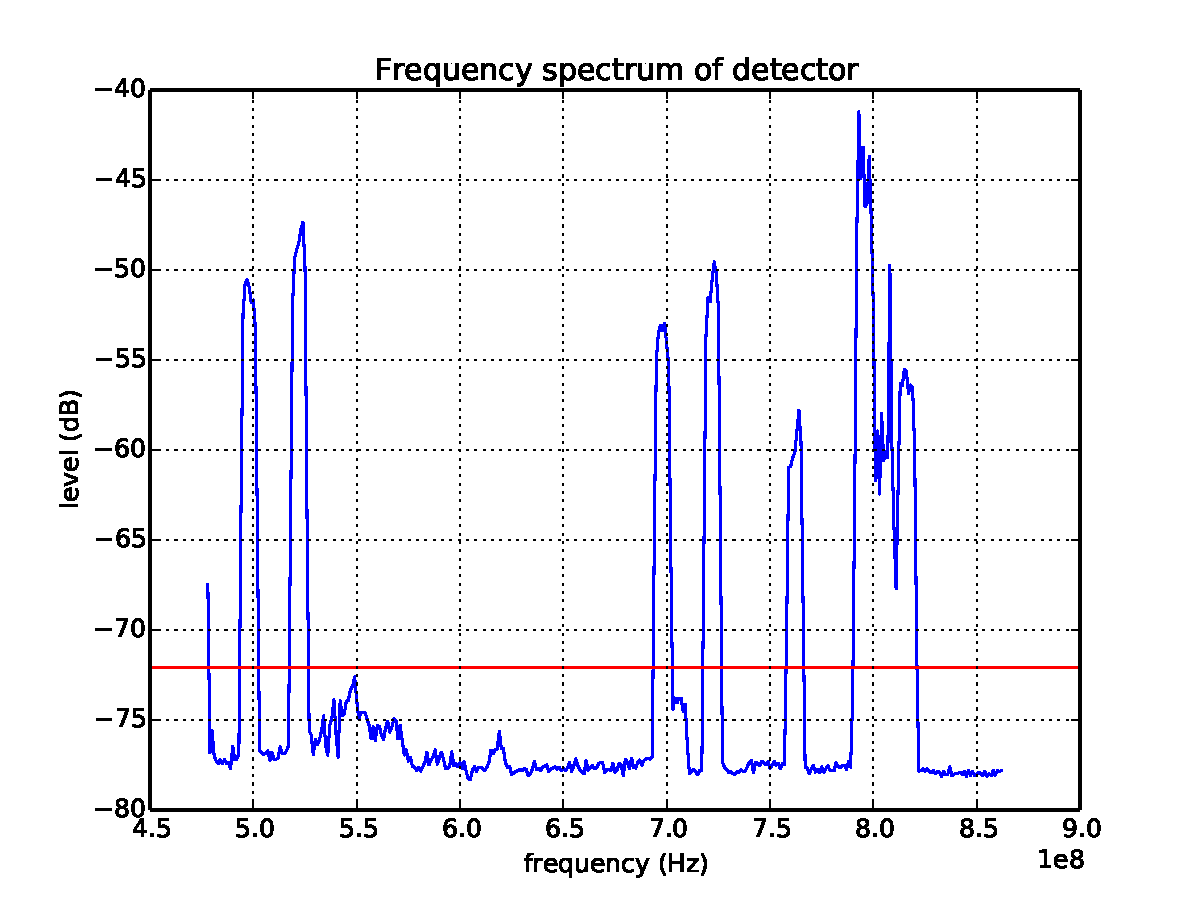
\includegraphics[width=\textwidth]{figures/lib-auto-freq}
    \end{subfigure}
    ~ %add desired spacing between images, e. g. ~, \quad, \qquad, \hfill etc. 
    %(or a blank line to force the subfigure onto a new line)
    \begin{subfigure}[b]{0.45\textwidth}
        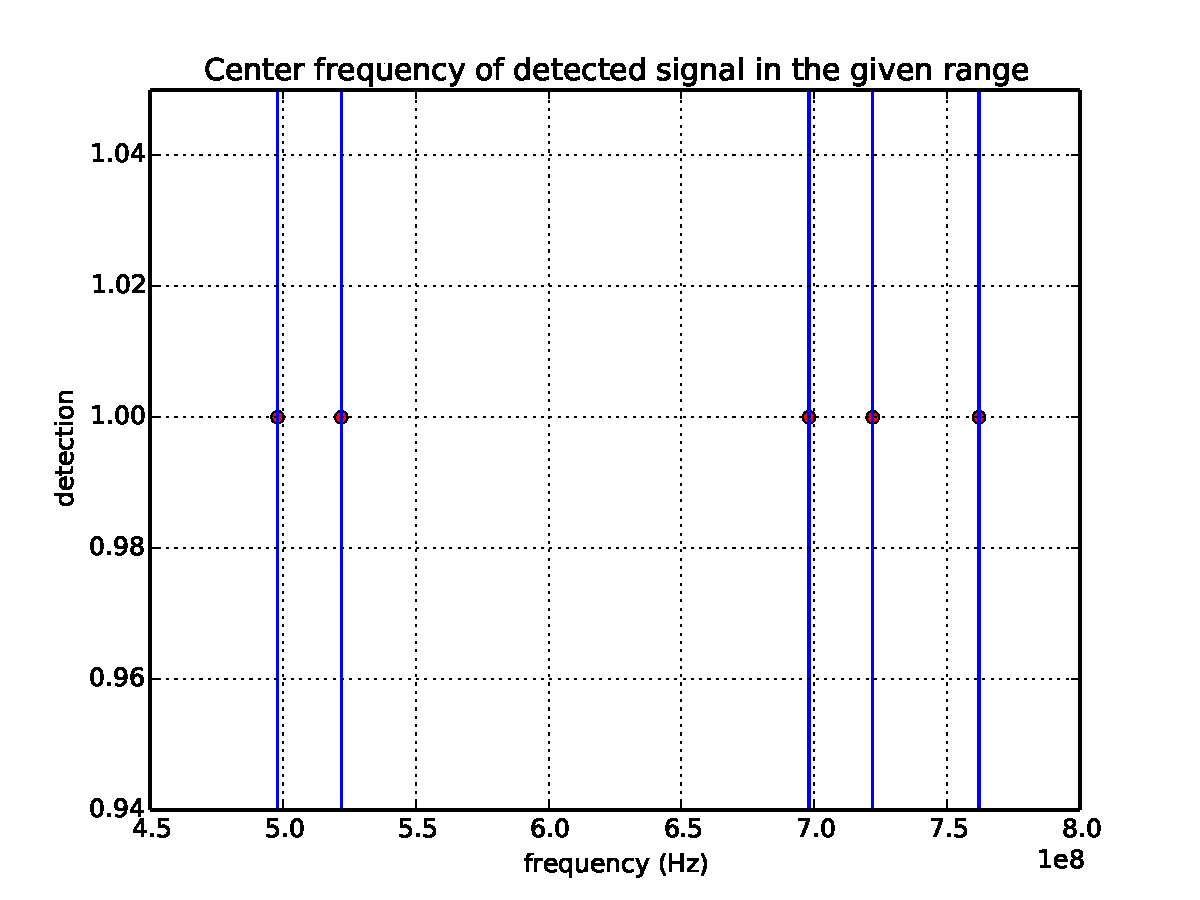
\includegraphics[width=\textwidth]{figures/lib-auto-center}
    \end{subfigure}
    \caption{Frequency spectrum of signal with automactic threshold finder (-72.0716 dB) captured at TU Delft Library}\label{fig:freq-lib-auto}
\end{figure}

The 480 MHz and 600 MHz signals have relatively high receive level with a bandwidth around 200 kHz. From the Nederland Frequency Database~\cite{robertelsinga2016}, those frequencies supposed to be empty. It could be caused by unregistered signal or probably the intermodulation product of other signals. Another interesting point is that the signal in the range of 790 - 820 MHz now become undetected though the level of the signal is sufficiently large. According to the same reference~\cite{robertelsinga2016}, this range is used for Wideband Frequency Modulation (WFM) radio. However, given the fact that the detector could detect these signals with sufficient threshold value, the final decision made by the detector will not be changed, again, because the bandwidth is far beyond 8 MHz. Moreover, in this project we are only interested in finding DVB-T signal spectrum. Thus, it should not be a problem to have misdetection on non-DVB-T signals.

The frequency spectrum of the second measurement done on different place, i.e. in Poptahof Noord, with threshold -60 dB is depicted in Figure~\ref{fig:popta-freq-60}. The signal spectrum is rather distinct from the frequency spectrum measured at TU Delft Library. Signal around 720 MHz has a stronger level but is still not considered as a DVB-T signal. Signal around 790 - 820 Mhz is detected as a single signal tough it seems like two signal appeared. However, this signal should not be considered as a DVB-T signal because it is a WFM radio signal. This indicates the false alarm generated by the detector.

% Poptahof results
\begin{figure}[H]
    \centering
    \begin{subfigure}[b]{0.45\textwidth}
        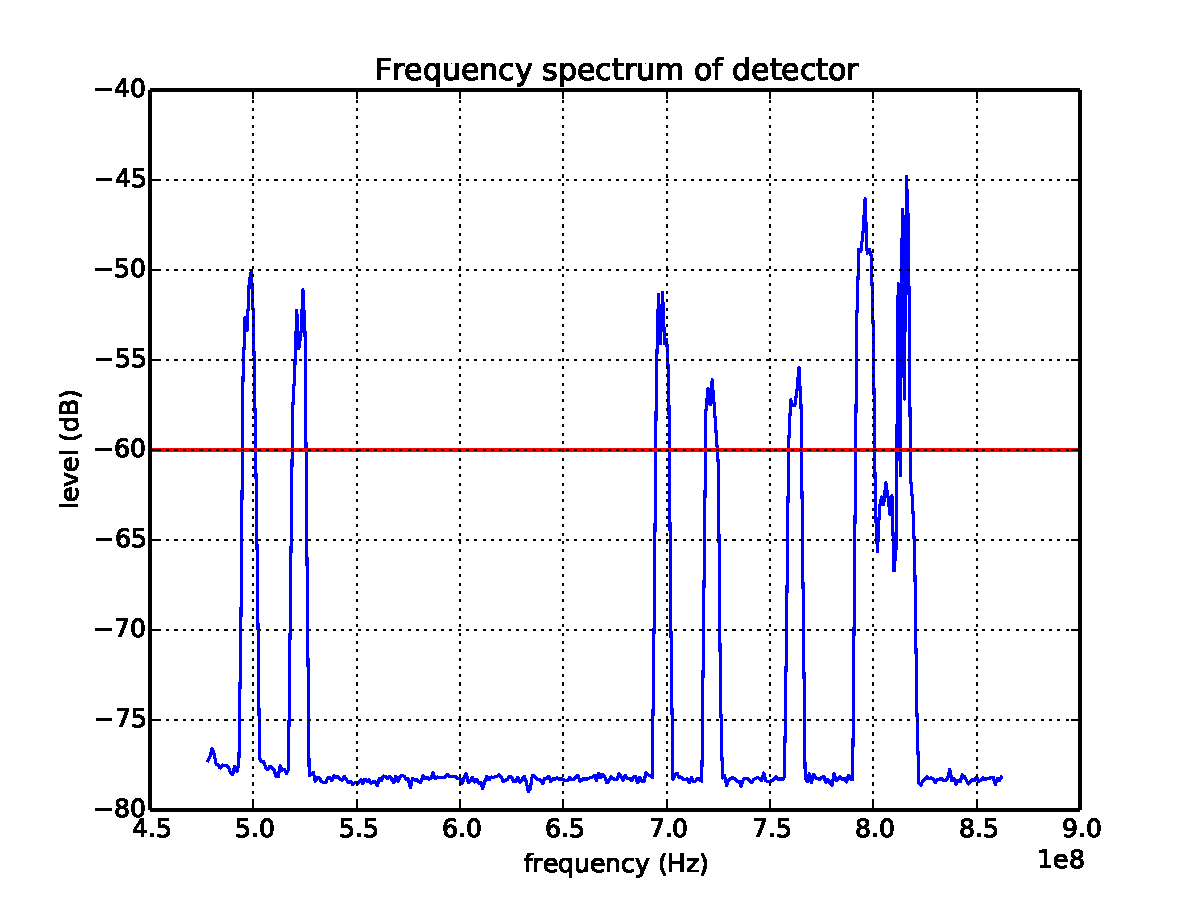
\includegraphics[width=\textwidth]{figures/popta-60-freq}
    \end{subfigure}
    ~ %add desired spacing between images, e. g. ~, \quad, \qquad, \hfill etc. 
    %(or a blank line to force the subfigure onto a new line)
    \begin{subfigure}[b]{0.45\textwidth}
        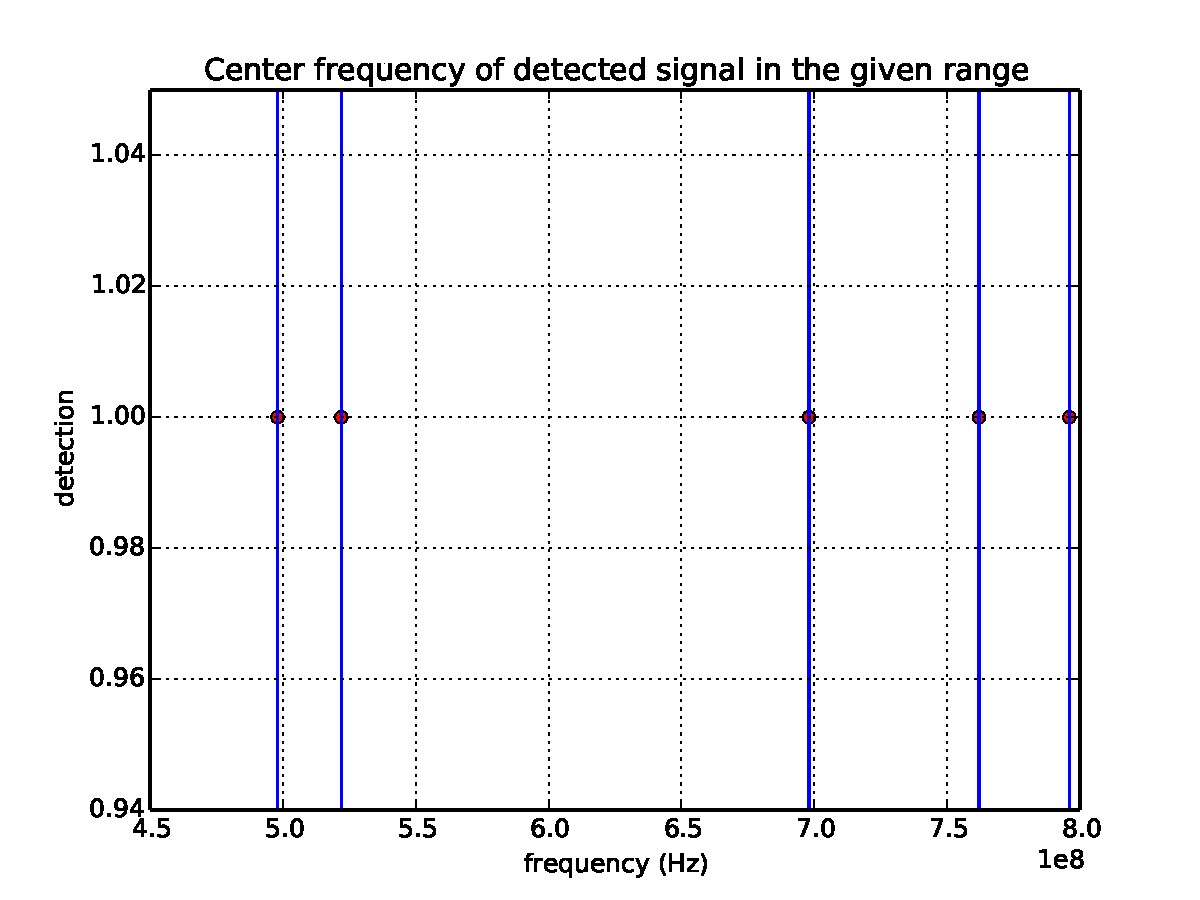
\includegraphics[width=\textwidth]{figures/popta-60-center}
    \end{subfigure}
    \caption{Frequency spectrum of signal with threshold -60 dB captured at Poptahof Noord}\label{fig:popta-freq-60}
\end{figure}

The automatic threshold finder has been used to get the lower threshold value. The results can be seen in Figure~\ref{fig:popta-freq-auto}. The difference is that the false alarm within the frequency range of 790 - 820 MHz has gone. The 722 MHz frequency (RTS Bouquet 1) could be detected properly. The result is the same as the previous result, which is measured at TU Delft Library.  In other words, the conditions of the channels could affect the detection depending on the threshold value being used.

\begin{figure}[H]
    \centering
    \begin{subfigure}[b]{0.45\textwidth}
        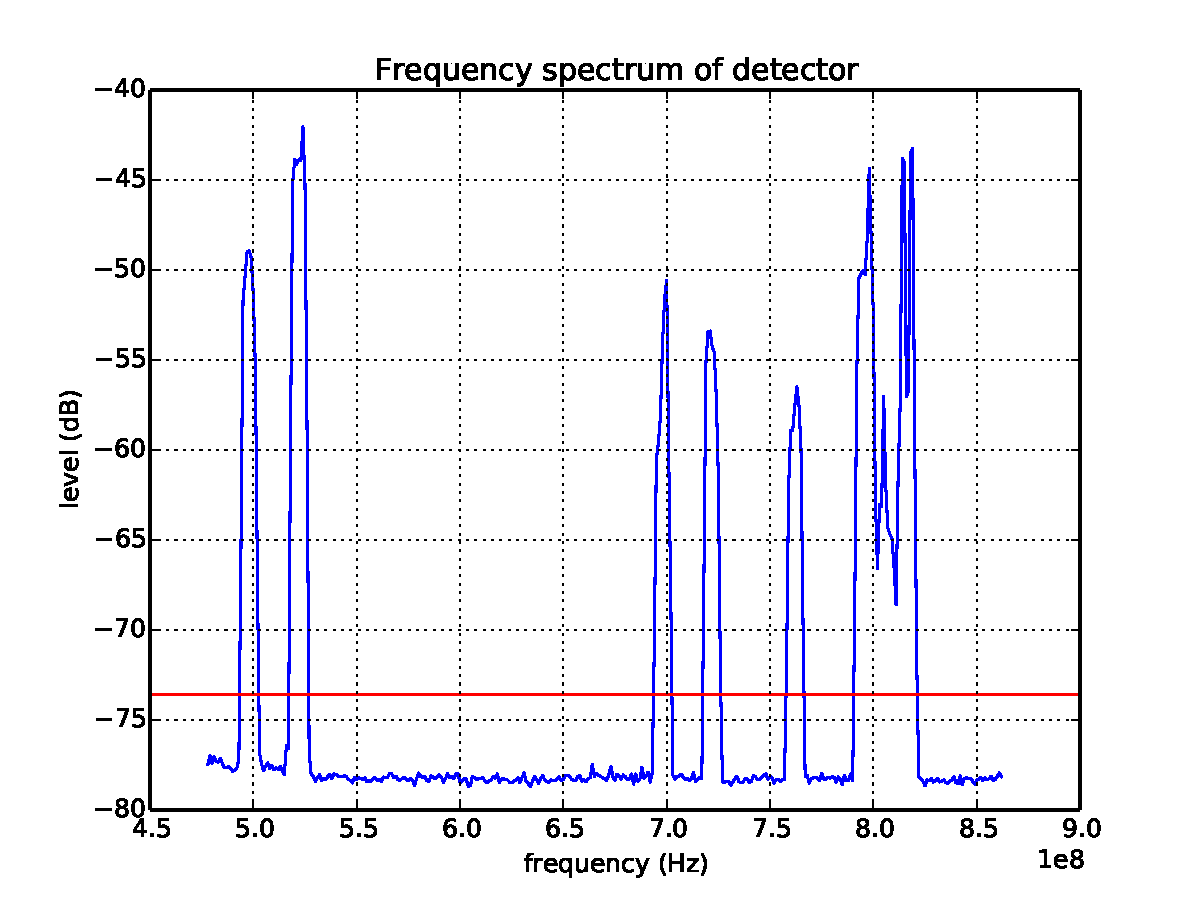
\includegraphics[width=\textwidth]{figures/popta-auto-freq}
    \end{subfigure}
    ~ %add desired spacing between images, e. g. ~, \quad, \qquad, \hfill etc. 
    %(or a blank line to force the subfigure onto a new line)
    \begin{subfigure}[b]{0.45\textwidth}
        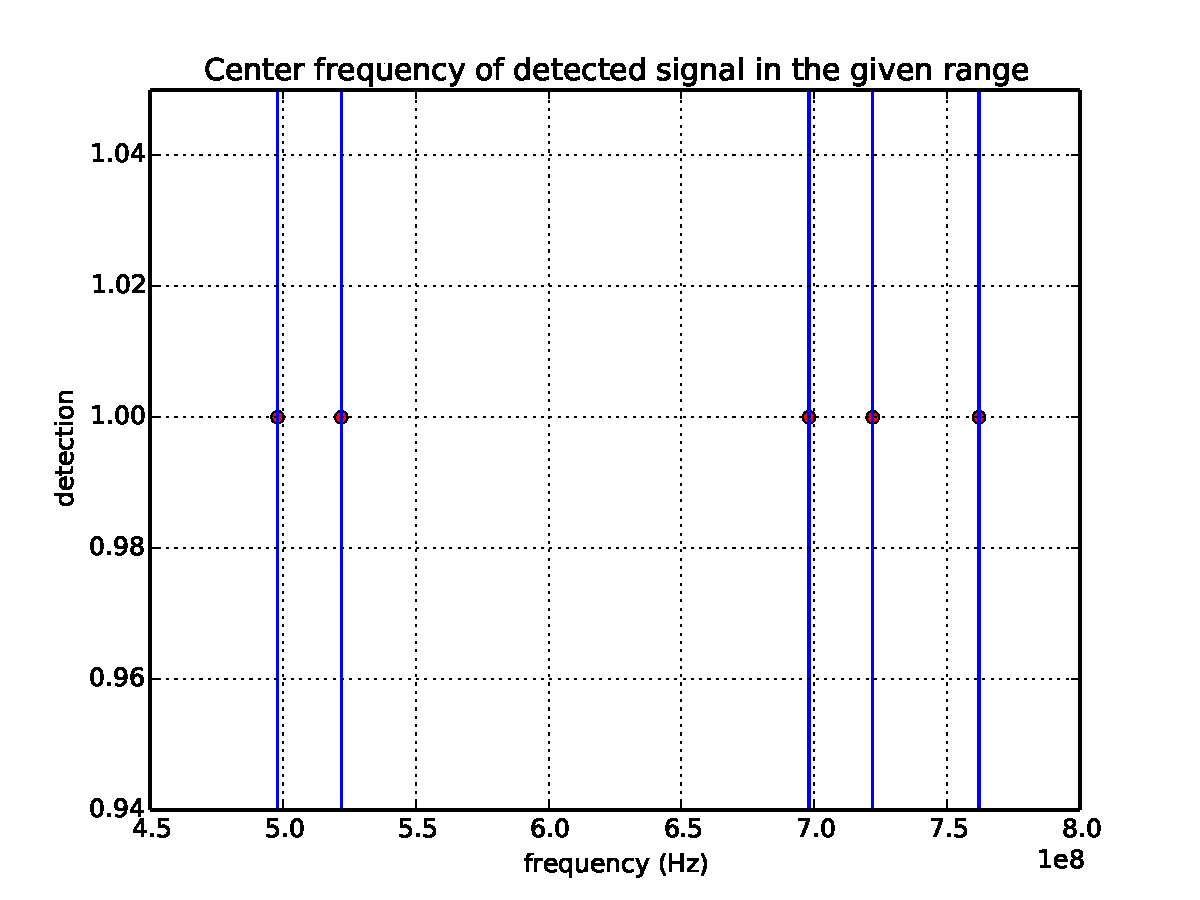
\includegraphics[width=\textwidth]{figures/popta-auto-center}
    \end{subfigure}
    \caption{Frequency spectrum of signal with automactic threshold finder (-73.5985 dB) captured at Poptahof Noord}\label{fig:popta-freq-auto}
\end{figure}

\section{Signal Misdetection}

Signal misdetection occurs whenever the detector could not be able to detect the presence of the signal due to the lack of the power level and lies below the threshold, or the bandwidth is beyond a certain value. For instance, Figure~\ref{fig:signal-misdetect} shows the unstable measurement at both edges of signal that has a center frequency of 722 MHz. Slightly changing the threshold value may lead to misdetection of the signal, see Figure~\ref{fig:popta-freq-60} and Figure~\ref{fig:popta-freq-auto} for comparison. To tackle this problem, we can decrease the threshold. Note that lowering the threshold could trigger a false alarm. Thus, the appropriate threshold value should be selected carefully. 

% Signal MisDetection at 722 MHz
\begin{figure}[H]
    \centering
    \begin{subfigure}[b]{0.45\textwidth}
        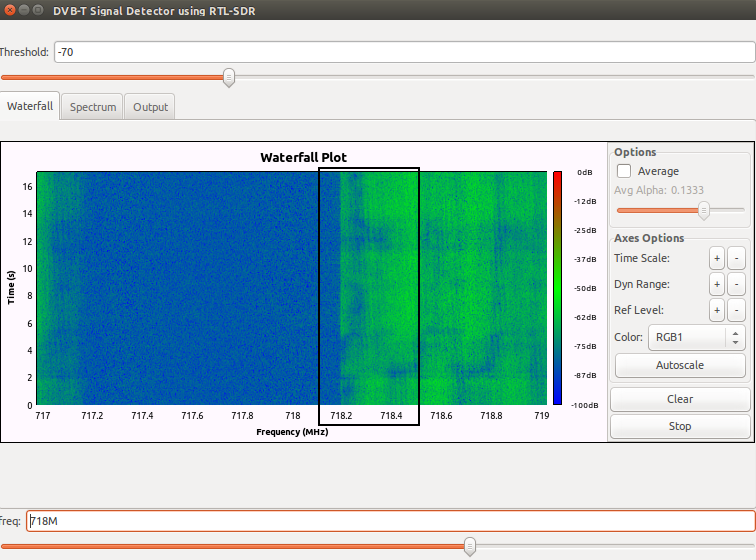
\includegraphics[width=\textwidth]{figures/misdetect-1}
    \end{subfigure}
    ~ %add desired spacing between images, e. g. ~, \quad, \qquad, \hfill etc. 
    %(or a blank line to force the subfigure onto a new line)
    \begin{subfigure}[b]{0.45\textwidth}
        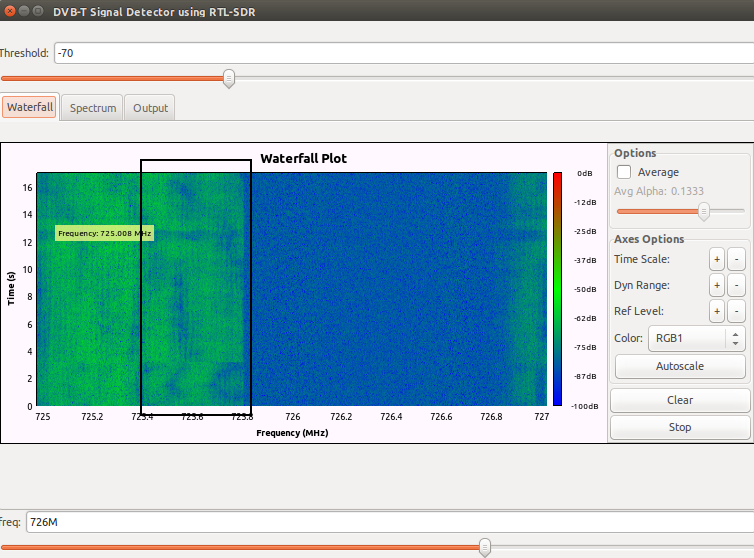
\includegraphics[width=\textwidth]{figures/misdetect-2}
    \end{subfigure}
    \caption{Waterfall plot of misdetected signal with center frequency 722 MHz and threshold -60 dB}\label{fig:signal-misdetect}
\end{figure}

\section{No Signal Presence}

The detector is said to detect an empty channel when it only senses a noise level. To detect average noise level, we can take several samples of measurement and calculate the distribution, typically in a form of normal distribution. Figure~\ref{fig:no-signal} shows the detection of an empty channel at the center frequency of 600 MHz. The blue color indicates low power level measurement or can be said as noise that lies around -78 dB. 

% No Signal presence at 600 MHz
\begin{figure}[H]
    \centering
    \begin{subfigure}[b]{0.45\textwidth}
        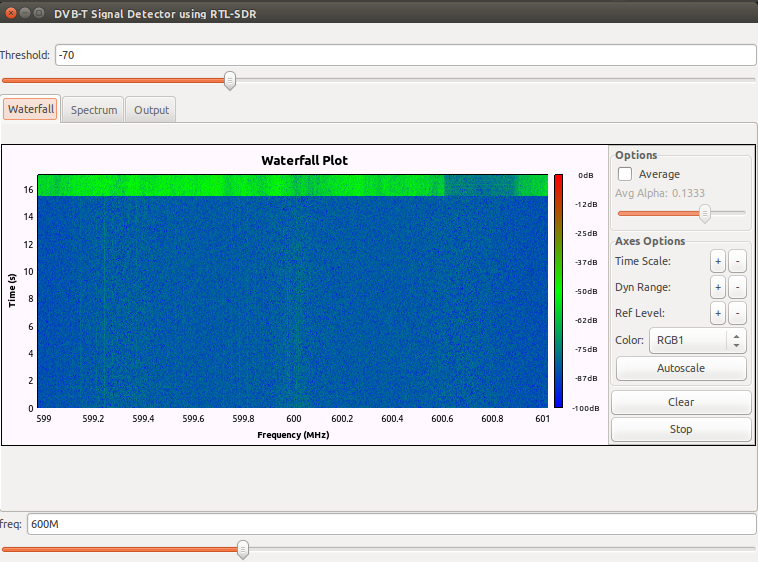
\includegraphics[width=\textwidth]{figures/no-signal-1}
    \end{subfigure}
    ~ %add desired spacing between images, e. g. ~, \quad, \qquad, \hfill etc. 
    %(or a blank line to force the subfigure onto a new line)
    \begin{subfigure}[b]{0.45\textwidth}
        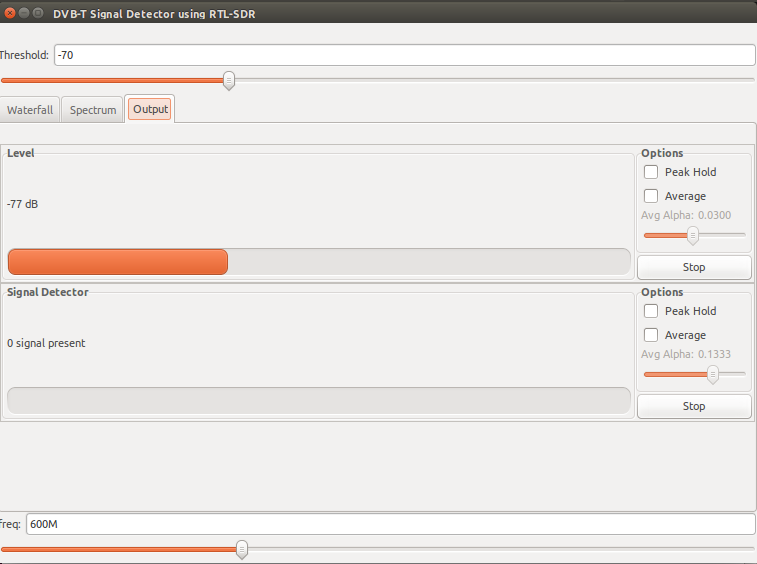
\includegraphics[width=\textwidth]{figures/no-signal-2}
    \end{subfigure}
    \caption{Waterfall plot of an empty channel with center frequency 600 MHz}\label{fig:no-signal}
\end{figure}

\section{False Alarm}

A false alarm occurs whenever the detector sense the presence of a signal though it supposed no to do so. The existence of carrier frequencies other than DVB-T can be one of the cause of false alarm. Moreover, the threshold value that is set nearly on the average of noise level may trigger false alarm once the noise level fluctuates and exceeds the threshold. One of the solutions is by increasing the threshold value. Figure X depicts the example of false alarm occurred at 790 - 820 MHz due to the exceeded number of bandwidth, i.e. non-DVB-T signal. See Figure~\ref{fig:freq-lib-60} and Figure~\ref{fig:freq-lib-auto} for comparison.

% False alarm at 790 - 820 MHz
\begin{figure}[H]
    \centering
    \begin{subfigure}[b]{0.45\textwidth}
        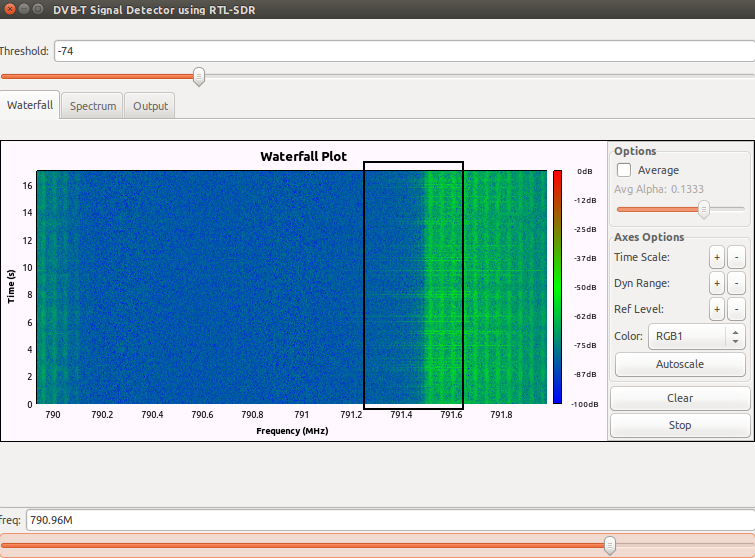
\includegraphics[width=\textwidth]{figures/false-alarm-1}
    \end{subfigure}
    ~ %add desired spacing between images, e. g. ~, \quad, \qquad, \hfill etc. 
    %(or a blank line to force the subfigure onto a new line)
    \begin{subfigure}[b]{0.45\textwidth}
        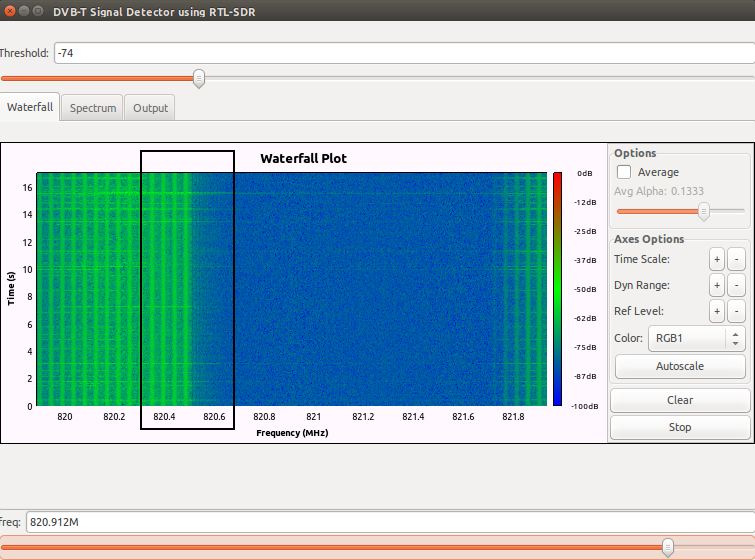
\includegraphics[width=\textwidth]{figures/false-alarm-2}
    \end{subfigure}
    \caption{Waterfall plot of signal on frequency range 780 - 820 MHz}\label{fig:no-signal}
\end{figure}

In this project, as we use a moving average block in GNU Radio Companion, the number of fluctuation of the detection is reducing a lot. Thus, it is probably hard to find a false alarm that comes from fluctuation of the noise level.

\section{Receiver Performance}

To analyze the receiver performance characteristic (ROC), first, we have created two probability density functions (PDF) that are combined into a single plot as seen in figure Figure~\ref{fig:all-pdf}, one from the measurement of detected signal, and one from the measurement of no empty channel. The PDF functions are generated based on the mean and the standard deviation of both type of measurements, see Table~\ref{tab:result-table}. From here, we can obtain the probability of detection and the probability of false alarm by taking the complement of cumulative distribution function (CDF) for each type of measurements. We have created a Python script to perform the ROC analysis easily. The result can be seen in Table~\ref{tab:prob-results}.

\begin{table}[H]
    \caption{Signal measurement results}
    \label{tab:prob-results}
    \resizebox{\textwidth}{!}{%
    \begin{tabular}{|p{0.15\textwidth}|p{0.15\textwidth}|p{0.2\textwidth}||p{0.15\textwidth}|p{0.15\textwidth}|p{0.2\textwidth}|}
    \hline
    \multicolumn{3}{|c||}{\textbf{TU Delft Library (6th floor) (52.002947, 4.375374)}} 			& \multicolumn{3}{|c|}{\textbf{Poptahof Noord (4th floor) (51.999881, 4.351265)}}	\\ \hline
    \textbf{Threshold (dB)} 	& 	\textbf{Probability of Detection (Pd)} 	&	\textbf{Probability of False Alarm (Pfa)}	& \textbf{Threshold (dB)} 	& \textbf{Probability of Detection (Pd)} & \textbf{Probability of False Alarm (Pfa)} \\ \hline \hline
    -72.0716    	&	0.9999586474               		&	0.3234032337                  		& -73.5985    		&  		0.9998543512               &  		0.3463925472                  \\ \hline
    -62				&  	0.9897364655               		&  	0.0264029694                  		& -62            	&  		0.9835587505               &  		0.0157515685                  \\ \hline
    \end{tabular}}%
\end{table}

% PDF using auto thereshold
\begin{figure}[H]
    \centering
    \begin{subfigure}[b]{0.45\textwidth}
        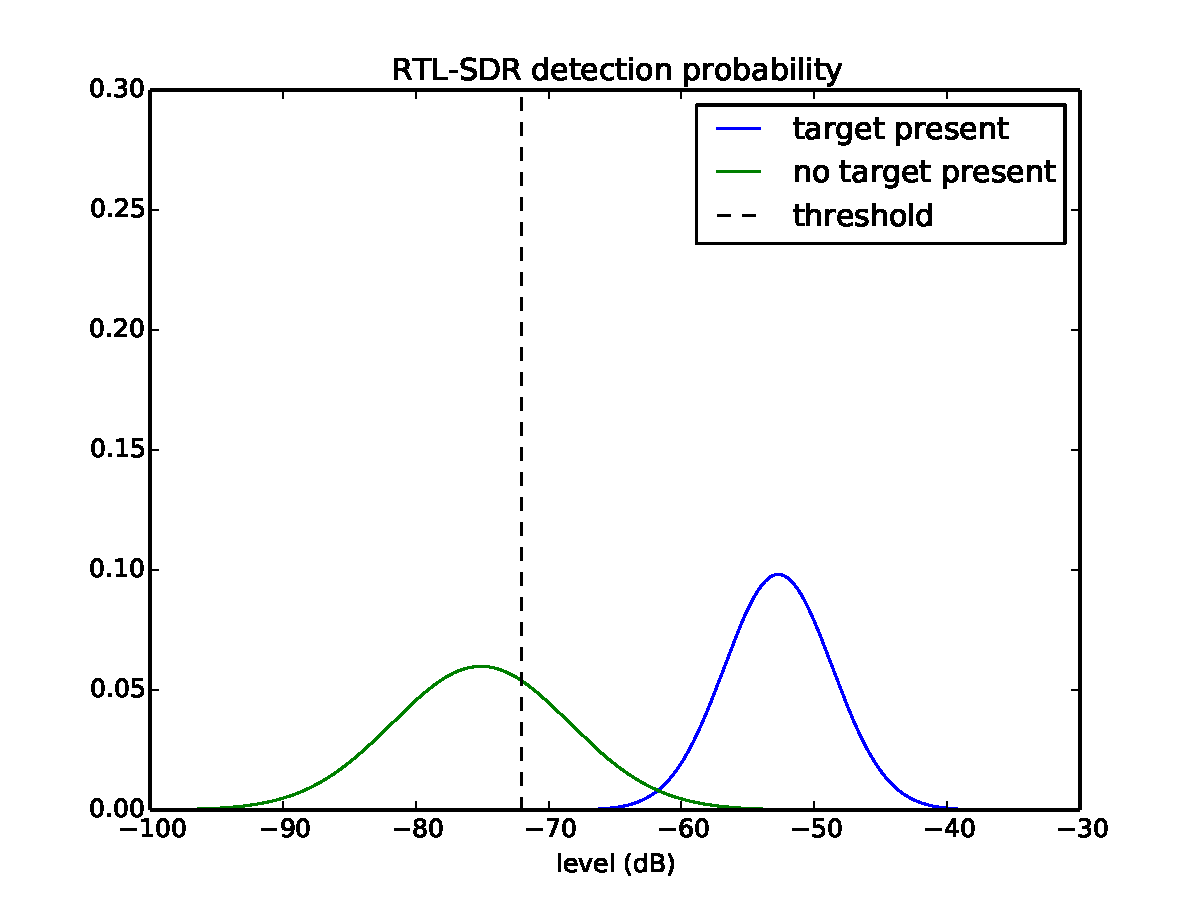
\includegraphics[width=\textwidth]{figures/lib-auto-pdf}
        \caption{TU Delft Library (threshold = -72.0716 dB)}
        \label{fig:lib-pdf}
    \end{subfigure}
    ~ %add desired spacing between images, e. g. ~, \quad, \qquad, \hfill etc. 
    %(or a blank line to force the subfigure onto a new line)
    \begin{subfigure}[b]{0.45\textwidth}
        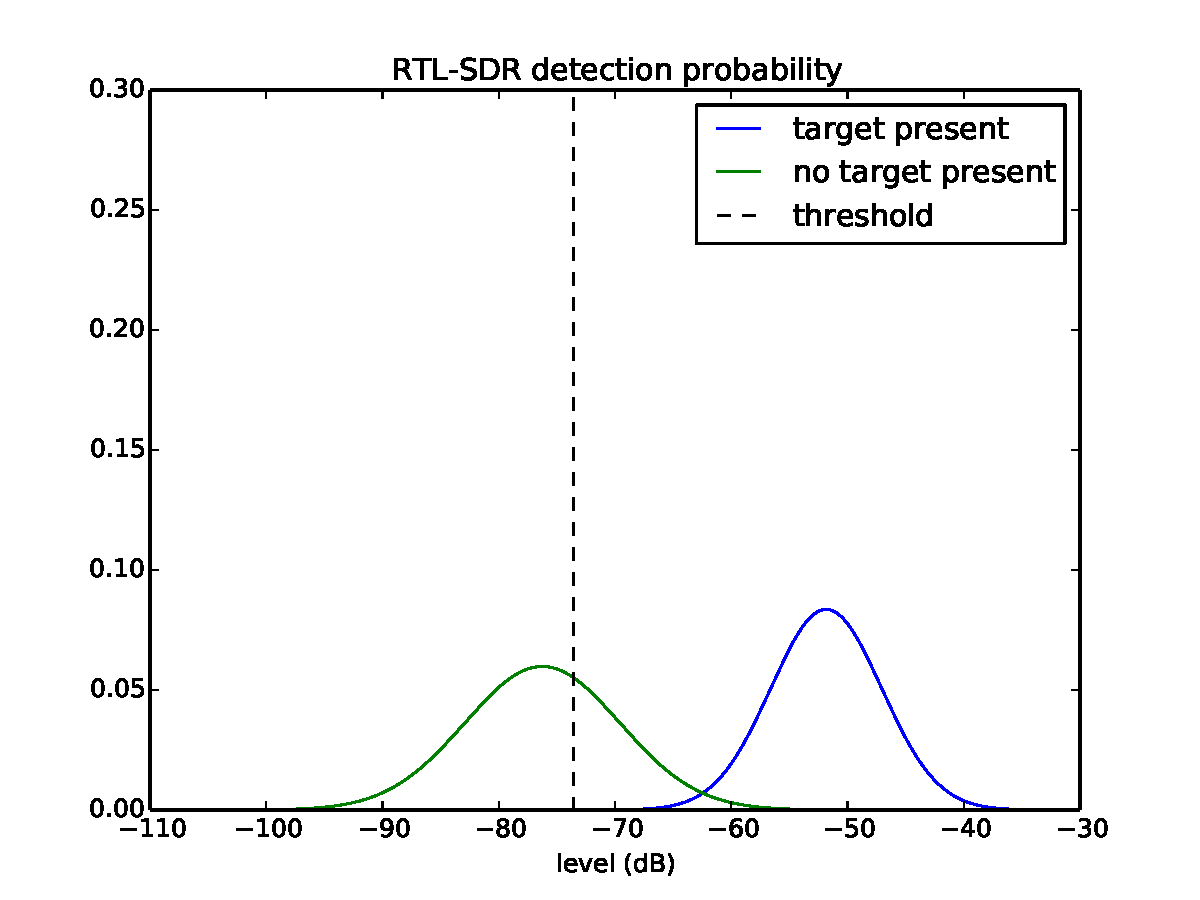
\includegraphics[width=\textwidth]{figures/popta-auto-pdf}
        \caption{Poptahof Noord (threshold = -73.5985 dB)}
        \label{fig:popta-pdf}
    \end{subfigure}
    \caption{Receiver performance measured at two different places}\label{fig:all-pdf}
\end{figure}

From Figure~\ref{fig:all-pdf} and Table~\ref{tab:prob-results}, despite that the probability of detection is sufficiently high, the probability of false alarm in two different places of measurements is still high. To get the optimal results, we can increase the threshold value to the point of intersection between the distribution of no target present and the distribution of target present. For both places, we obtain around -62 dB as the optimal threshold. Figure~\ref{fig:all-pdf-optimized} depicts the optimized threshold value in the PDFs.

% PDF using auto thereshold optimized
\begin{figure}[H]
    \centering
    \begin{subfigure}[b]{0.45\textwidth}
        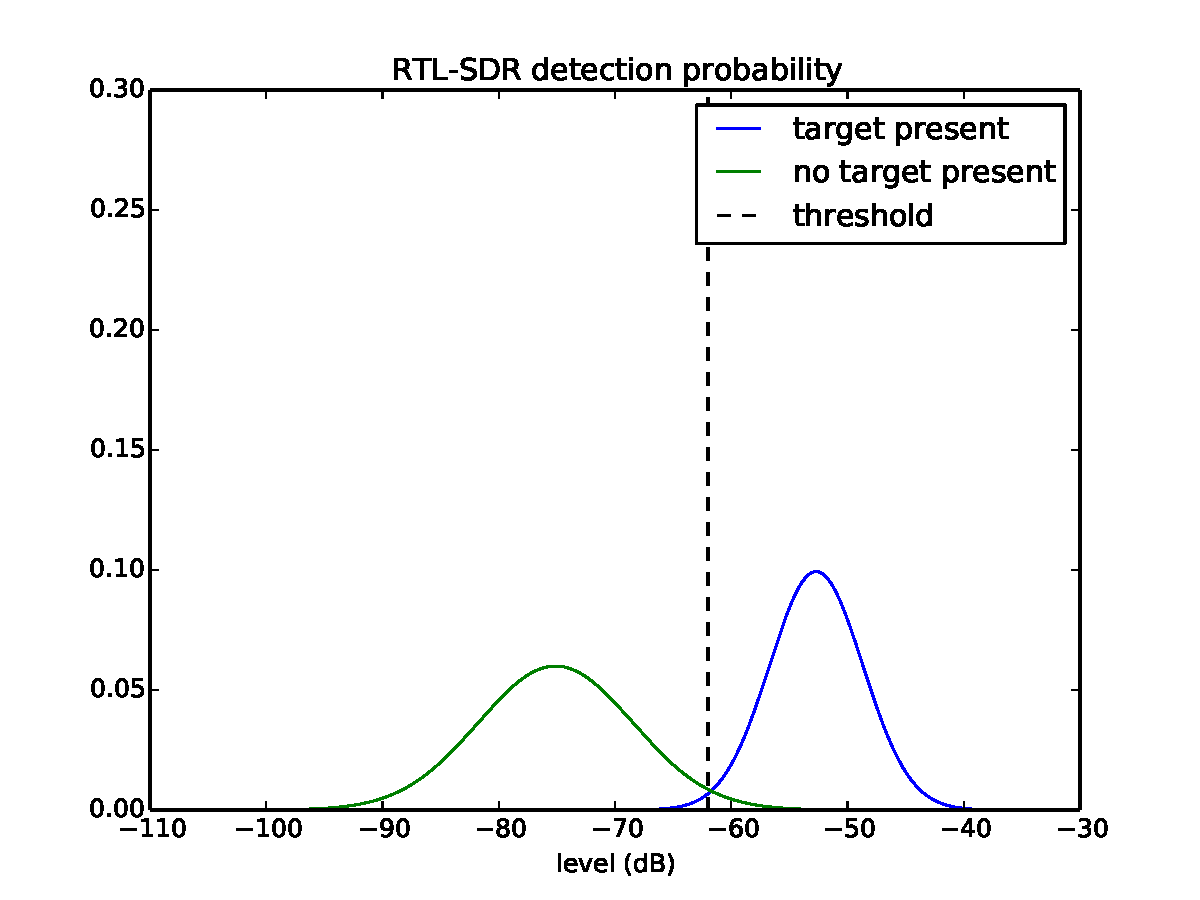
\includegraphics[width=\textwidth]{figures/lib-optim-pdf}
        \caption{TU Delft Library (threshold = -62 dB)}
        \label{fig:lib-pdf-optim}
    \end{subfigure}
    ~ %add desired spacing between images, e. g. ~, \quad, \qquad, \hfill etc. 
    %(or a blank line to force the subfigure onto a new line)
    \begin{subfigure}[b]{0.45\textwidth}
        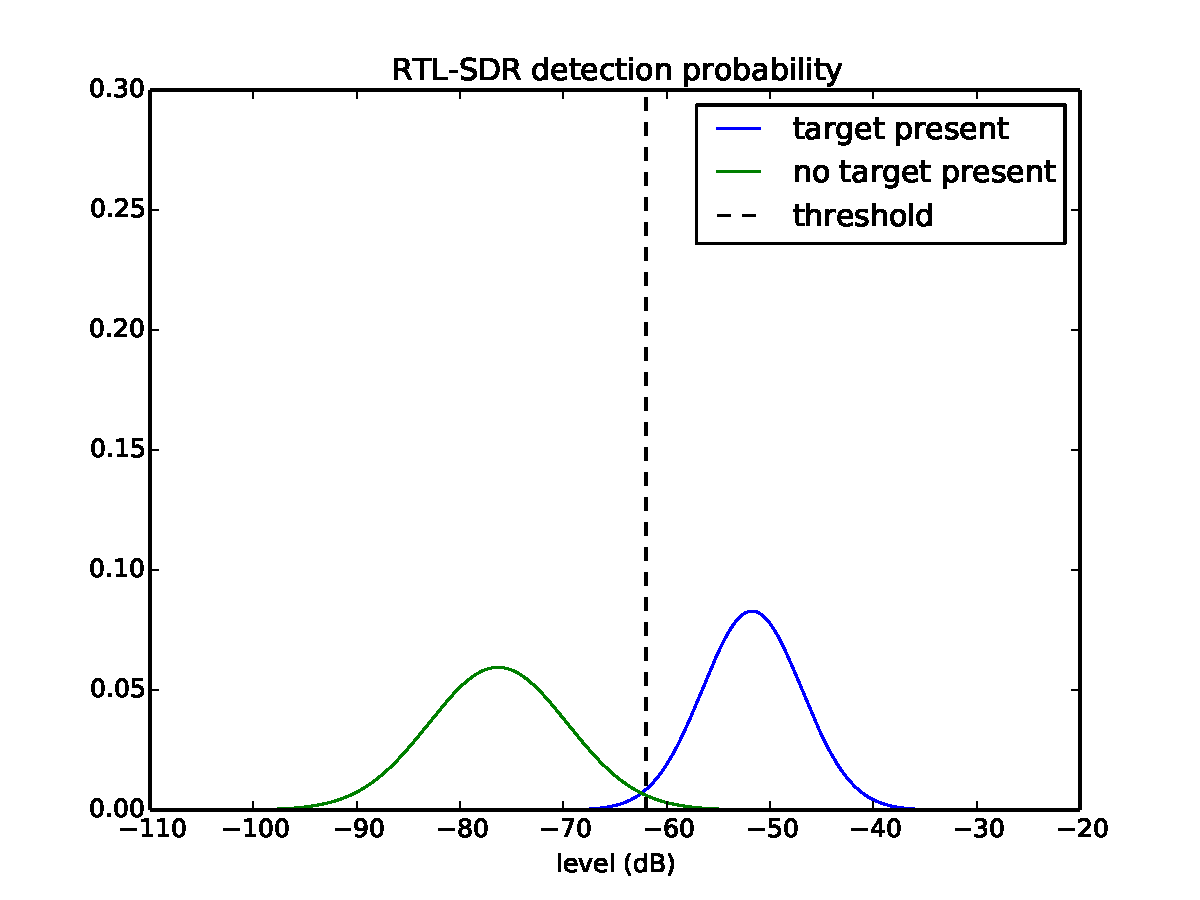
\includegraphics[width=\textwidth]{figures/popta-optim-pdf}
        \caption{Poptahof Noord (threshold = -62 dB)}
        \label{fig:popta-pdf-optim}
    \end{subfigure}
    \caption{Optimal threshold value of receiver performance measured at two different places}\label{fig:all-pdf-optimized}
\end{figure}

Based on the PDF of detection and false alarm, we can obtain ROC curve with probability of false alarm (Pfa) on the horizontal axis and probability of detection (Pd) on the vertical axis. The ROC curve is depicted in Figure~\ref{fig:roc-combine}. Note that the working area of the receiver lies below the ROC curve.

% ROC combine
\begin{figure}[H]
    \centering
    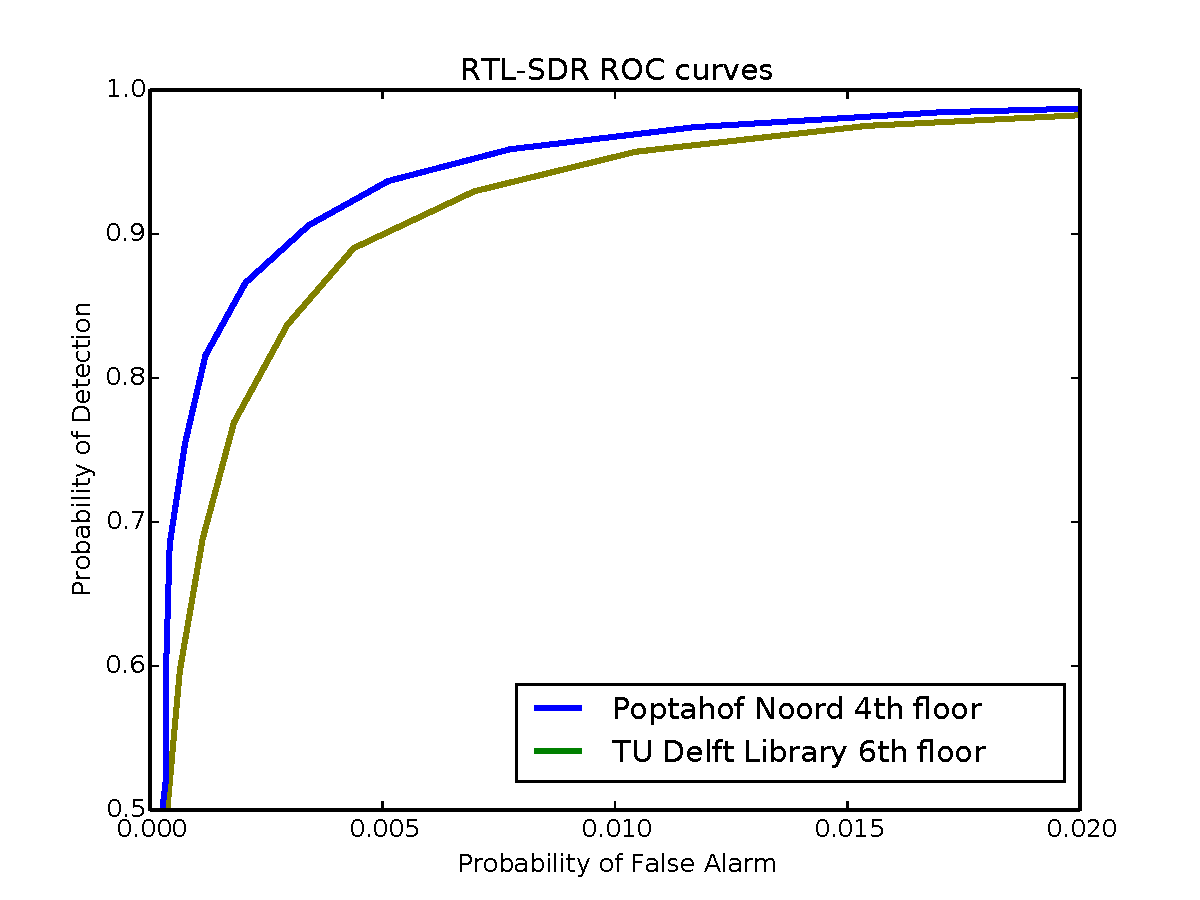
\includegraphics[width=0.8\textwidth]{figures/lib-roc-combine}
    \caption{ROC curve of the receiver measured at two different places}\label{fig:roc-combine}
\end{figure}

In Figure~\ref{fig:roc-combine}, there is a difference between the curve obtained from the measurement at TU Delft and the measurement at Poptahof Noord. This indicates that the detector or receiver characteristic depends on the channels conditions, e.g. noise level, SNR, line of sight, and weather. The lower the probability of false alarm followed by the increasing probability of detection, the better the detector is.